\chapter{روش‌شناسی و طراحی مدل}

\section{انتخاب مدل‌ها و منطق طراحی}
با توجه به ماهیت داده‌ها و چالش‌های موجود در تشخیص باج‌افزار، سه خانواده الگوریتم با دقت مورد ارزیابی و انتخاب قرار گرفتند. این انتخاب بر اساس مطالعات پیشین، ویژگی‌های داده‌های حاضر و نیازمندی‌های خاص تشخیص باج‌افزار انجام شده است. هر یک از این مدل‌ها مزایا و کاربردهای منحصربه‌فردی ارائه می‌دهند که در ادامه به تفصیل بررسی شده‌اند.

\subsection{معیارهای انتخاب مدل‌ها}
\begin{itemize}
    \item \textbf{رندوم فارست \lr{(Random Forest)}}:
    \begin{itemize}
        \item مقاومت بالا در برابر نویز و داده‌های پرت که در تحلیل رفتار فایل‌ها بسیار رایج است
        \item توانایی پردازش داده‌های با ابعاد زیاد بدون نیاز به پیش‌پردازش‌های پیچیده
        \item ارائه اهمیت ذاتی ویژگی‌ها برای تفسیر بهتر نتایج و شناسایی الگوهای کلیدی در رفتار باج‌افزارها
        \item عملکرد خوب با مجموعه داده‌های کوچک تا متوسط (مانند مجموعه داده حاضر)
        \item کاهش احتمال بیش‌برازش با استفاده از میانگین‌گیری از چندین درخت تصمیم مستقل
    \end{itemize}

    \item \textbf{XGBoost}:
    \begin{itemize}
        \item پشتیبانی از داده‌های نامتوازن با استفاده از پارامتر \lr{scale\_pos\_weight} که برای مسئله تشخیص باج‌افزار (با تعداد نمونه‌های مثبت کمتر) بسیار مفید است
        \item بهینه‌سازی مبتنی بر گرادیان تقویتی برای دستیابی به دقت بالا در طبقه‌بندی
        \item امکان اجرای موازی (با استفاده از GPU در صورت نیاز) برای کاهش زمان آموزش در مدل‌های پیچیده
        \item قابلیت تنظیم دقیق مدل با استفاده از هرس درخت برای جلوگیری از بیش‌برازش
        \item مقیاس‌پذیری بالا با داده‌های بزرگ و ویژگی‌های متنوع
    \end{itemize}

    \item \textbf{شبکه عصبی چندلایه (MLP)}:
    \begin{itemize}
        \item توانایی یادگیری روابط غیرخطی پیچیده بین ویژگی‌های رفتاری فایل‌ها
        \item قابلیت توسعه به معماری‌های عمیق‌تر در صورت افزایش حجم داده در آینده
        \item انعطاف‌پذیری بالا در ترکیب انواع ویژگی‌های عددی و کدگذاری‌شده
        \item یادگیری خودکار ویژگی‌های سطح بالاتر \lr{(feature learning)} از داده‌های خام
        \item توانایی مدل‌سازی الگوهای پیچیده و مخفی در داده‌ها که ممکن است در روش‌های سنتی قابل شناسایی نباشند
    \end{itemize}
\end{itemize}

\subsection{مقایسه تئوریک مدل‌ها}
انتخاب نهایی مدل‌ها بر اساس تحلیل نقاط قوت و ضعف هر الگوریتم در زمینه تشخیص باج‌افزار صورت گرفته است. جدول زیر مقایسه‌ای از این ویژگی‌ها ارائه می‌دهد:

\begin{table}[h]
    \centering
    \begin{tabular}{|p{3cm}|p{3.5cm}|p{3.5cm}|p{3.5cm}|}
        \hline
        \textbf{معیار} & \textbf{رندوم فارست} & \textbf{XGBoost} & \textbf{شبکه عصبی (MLP)} \\ \hline
        کارایی با داده‌های کم & عالی & خوب & متوسط \\ \hline
        سرعت آموزش & سریع (قابل موازی‌سازی) & متوسط & کُند \\ \hline
        مقاومت در برابر بیش‌برازش & بالا & متوسط (با هرس مناسب) & پایین (نیازمند تنظیم دقیق) \\ \hline
        تفسیرپذیری & بالا & متوسط & پایین \\ \hline
        توانایی یادگیری الگوهای پیچیده & متوسط & بالا & بسیار بالا \\ \hline
        نیاز به پیش‌پردازش داده & کم & کم & زیاد \\ \hline
    \end{tabular}
    \caption{مقایسه تئوریک مدل‌های انتخاب‌شده}
\end{table}

\section{فرآیند آموزش و بهینه‌سازی}
در این بخش، روند آموزش مدل‌ها، استراتژی‌های اعتبارسنجی و تنظیم هایپرپارامترها به تفصیل شرح داده شده است. فرآیند آموزش به‌صورت سیستماتیک و با رویکرد علمی طراحی گردیده تا از اعتبار نتایج اطمینان حاصل شود.

\subsection{آماده‌سازی داده‌ها برای آموزش}
قبل از آموزش مدل‌ها، مجموعه داده تحت پردازش‌های زیر قرار گرفت:

\begin{itemize}
    \item \textbf{نرمال‌سازی ویژگی‌ها:} تمامی ویژگی‌های عددی با استفاده از روش \lr{Min-Max Scaling} در بازه $[0, 1]$ نرمال‌سازی شدند تا تأثیر مقیاس ویژگی‌ها بر عملکرد مدل‌ها کاهش یابد.

    \item \textbf{کدگذاری ویژگی‌های کیفی:} ویژگی‌های کیفی مانند نوع فایل و دسته‌بندی با استفاده از روش \lr{One-Hot Encoding} کدگذاری شدند.

    \item \textbf{مدیریت عدم توازن داده‌ها:} با توجه به نسبت نامتوازن بین فایل‌های سالم و باج‌افزار (۳۵۴ به ۱۱۹)، از روش‌های زیر برای متعادل‌سازی استفاده شد:
    \begin{itemize}
        \item استفاده از تکنیک \lr{SMOTE} برای ایجاد نمونه‌های مصنوعی از کلاس اقلیت
        \item تنظیم وزن کلاس‌ها در مدل‌های پشتیبانی‌کننده (مانند پارامتر \lr{class\_weight} در رندوم فارست)
        \item تنظیم پارامتر \lr{scale\_pos\_weight} در XGBoost متناسب با نسبت عدم توازن داده‌ها
    \end{itemize}
\end{itemize}

\subsection{استراتژی اعتبارسنجی}
برای ارزیابی پایدار و قابل اعتماد عملکرد مدل‌ها، از استراتژی‌های زیر استفاده شده است:

\begin{itemize}
    \item \textbf{تقسیم داده:} داده‌ها به نسبت ۶۰٪ آموزش، ۲۰٪ اعتبارسنجی و ۲۰٪ آزمون تقسیم شدند. مجموعه اعتبارسنجی برای تنظیم هایپرپارامترها استفاده شد، در حالی که مجموعه آزمون صرفاً برای ارزیابی نهایی مدل‌ها مورد استفاده قرار گرفت.

    \item \textbf{اعتبارسنجی متقابل:} از روش \lr{Stratified K-Fold Cross-Validation} با $k=5$ استفاده شد تا توزیع متوازنی از کلاس‌ها در هر تقسیم وجود داشته باشد. این روش به‌ویژه برای مجموعه داده‌های نامتوازن مفید است.

    \item \textbf{اولویت‌بندی معیارها:} با توجه به اهمیت بالای تشخیص صحیح باج‌افزارها (کلاس اقلیت)، معیارهای زیر با اولویت بالاتری مورد توجه قرار گرفتند:
    \begin{itemize}
        \item \lr{Recall} (حساسیت): برای اطمینان از شناسایی حداکثری باج‌افزارها
        \item \lr{F1-Score}: برای برقراری تعادل بین دقت و حساسیت
        \item \lr{Area Under Precision-Recall Curve (AUPRC)}: معیاری مناسب برای داده‌های نامتوازن
    \end{itemize}

    \item \textbf{تکنیک‌های مقابله با بیش‌برازش:} برای جلوگیری از بیش‌برازش، روش‌های زیر به کار گرفته شدند:
    \begin{itemize}
        \item \lr{Early Stopping} در آموزش مدل‌ها با نظارت بر عملکرد در مجموعه اعتبارسنجی
        \item استفاده از تنظیم‌کننده‌های \lr{L1} و \lr{L2} در شبکه عصبی
        \item پیاده‌سازی \lr{Dropout} با نرخ ۰.۳ در لایه‌های شبکه عصبی
    \end{itemize}
\end{itemize}

\subsection{بهینه‌سازی هایپرپارامترها}
تنظیم بهینه هایپرپارامترها نقش بسزایی در عملکرد مدل‌ها دارد. در این پژوهش، از روش‌های جستجوی سیستماتیک برای یافتن بهترین ترکیب پارامترها استفاده شده است:

\begin{itemize}
    \item \textbf{جستجوی شبکه‌ای (\lr{Grid Search}):} برای مدل‌های با تعداد هایپرپارامتر کمتر (مانند رندوم فارست) از روش جستجوی شبکه‌ای استفاده شد که تمام ترکیب‌های ممکن پارامترها را ارزیابی می‌کند.

    \item \textbf{جستجوی تصادفی (\lr{Random Search}):} برای مدل‌های با فضای هایپرپارامتر بزرگتر (مانند شبکه عصبی) از جستجوی تصادفی با ۱۰۰ تکرار استفاده شد که نسبت به جستجوی شبکه‌ای کارآمدتر است.

    \item \textbf{جستجوی بیزی (\lr{Bayesian Optimization}):} برای تنظیم دقیق‌تر پارامترهای XGBoost از روش بهینه‌سازی بیزی استفاده شد که با استفاده از مدل احتمالاتی، فضای جستجو را هوشمندانه کاوش می‌کند.
\end{itemize}

جدول زیر محدوده‌های بهینه‌سازی و مقادیر نهایی انتخاب‌شده برای هایپرپارامترهای اصلی هر مدل را نشان می‌دهد:

\begin{table}[h]
    \centering
    \begin{tabular}{|l|l|l|l|}
        \hline
        \textbf{مدل} & \textbf{پارامتر} & \textbf{محدوده جستجو} & \textbf{مقدار بهینه} \\ \hline
        \multirow{4}{*}{رندوم فارست} & \lr{n\_estimators} & ۵۰، ۱۰۰، ۲۰۰، ۳۰۰، ۵۰۰ & ۳۰۰ \\ \cline{2-4}
        & \lr{max\_depth} & ۵، ۱۰، ۱۵، ۲۰، None & ۱۵ \\ \cline{2-4}
        & \lr{min\_samples\_split} & ۲، ۵، ۱۰ & ۵ \\ \cline{2-4}
        & \lr{min\_samples\_leaf} & ۱، ۲، ۴ & ۲ \\ \hline
        \multirow{5}{*}{XGBoost} & \lr{max\_depth} & ۳-۱۰ & ۶ \\ \cline{2-4}
        & \lr{learning\_rate} & ۰.۰۱-۰.۳ & ۰.۰۵ \\ \cline{2-4}
        & \lr{n\_estimators} & ۵۰-۵۰۰ & ۲۵۰ \\ \cline{2-4}
        & \lr{subsample} & ۰.۶-۱.۰ & ۰.۸ \\ \cline{2-4}
        & \lr{colsample\_bytree} & ۰.۶-۱.۰ & ۰.۷۵ \\ \hline
        \multirow{5}{*}{شبکه عصبی (MLP)} & \lr{hidden\_layer\_sizes} & [(۶۴), (۱۲۸), (۶۴,۳۲), (۱۲۸,۶۴)] & (۱۲۸,۶۴) \\ \cline{2-4}
        & \lr{activation} & [relu, tanh] & relu \\ \cline{2-4}
        & \lr{learning\_rate} & ۰.۰۰۱-۰.۱ & ۰.۰۰۵ \\ \cline{2-4}
        & \lr{alpha} (L2 penalty) & ۰.۰۰۰۱-۰.۰۱ & ۰.۰۰۱ \\ \cline{2-4}
        & \lr{batch\_size} & [۳۲, ۶۴, ۱۲۸] & ۶۴ \\ \hline
    \end{tabular}
    \caption{محدوده‌های بهینه‌سازی و مقادیر نهایی هایپرپارامترها}
\end{table}

\subsection{جزئیات پیاده‌سازی}
پیاده‌سازی مدل‌ها با استفاده از کتابخانه‌های زیر در زبان برنامه‌نویسی پایتون انجام شد:

\begin{itemize}
    \item \textbf{Scikit-learn} برای پیاده‌سازی مدل رندوم فارست، پیش‌پردازش داده‌ها و ارزیابی عملکرد
    \item \textbf{XGBoost} برای پیاده‌سازی مدل XGBoost با تنظیمات بهینه
    \item \textbf{Keras با پشتیبانی از تنسورفلو:} برای ساخت و آموزش مدل شبکه عصبی
    \item \textbf{Pandas و NumPy} برای مدیریت و پردازش داده‌ها
    \item \textbf{Matplotlib و Seaborn} برای تجسم نتایج و تحلیل‌های آماری
\end{itemize}


\section{نتایج اولیه و ارزیابی عملکرد}
پس از آموزش مدل‌ها با پارامترهای بهینه، عملکرد آن‌ها بر روی مجموعه آزمون با استفاده از معیارهای مختلف ارزیابی شد. این ارزیابی جامع، امکان مقایسه منصفانه بین مدل‌های مختلف را فراهم می‌کند.

\subsection{معیارهای ارزیابی مورد استفاده}
برای ارزیابی عملکرد مدل‌ها، علاوه بر معیارهای رایج مانند دقت (Accuracy)، از معیارهای تخصصی‌تر زیر نیز استفاده شده است:

\begin{itemize}
    \item \textbf{دقت (Precision):} نسبت پیش‌بینی‌های صحیح مثبت به کل پیش‌بینی‌های مثبت
    \item \textbf{حساسیت (Recall):} نسبت پیش‌بینی‌های صحیح مثبت به کل نمونه‌های مثبت واقعی
    \item \textbf{F1-Score:} میانگین هارمونیک دقت و حساسیت
    \item \textbf{ROC AUC:} سطح زیر منحنی مشخصه عملکرد گیرنده
    \item \textbf{Average Precision:} میانگین وزنی دقت‌ها در هر سطح از حساسیت
    \item \textbf{زمان استنتاج:} زمان لازم برای پیش‌بینی کلاس نمونه‌های آزمون
\end{itemize}

\subsection{مقایسه عملکرد مدل‌ها}
جدول زیر مقایسه‌ای جامع از عملکرد مدل‌های مختلف بر روی مجموعه آزمون ارائه می‌دهد:

\begin{table}[h]
    \centering
    \begin{tabular}{|l|c|c|c|c|c|c|}
        \hline
        \textbf{مدل} & \textbf{دقت} & \textbf{حساسیت} & \textbf{F1-Score} & \textbf{ROC AUC} & \textbf{Avg. Precision} & \textbf{زمان استنتاج (ms)} \\ \hline
        رندوم فارست & 0.98 & 0.96 & 0.97 & 0.99 & 0.95 & 8.2 \\ \hline
        XGBoost & 0.97 & 0.98 & 0.96 & 0.985 & 0.94 & 5.4 \\ \hline
        شبکه عصبی (MLP) & 0.94 & 0.95 & 0.93 & 0.981 & 0.96 & 12.7 \\ \hline
    \end{tabular}
    \caption{مقایسه جامع عملکرد مدل‌های پیشنهادی}
\end{table}

\subsection{تحلیل ماتریس درهم‌ریختگی (Confusion Matrix)}
برای درک بهتر عملکرد مدل‌ها، ماتریس درهم‌ریختگی هر یک از آن‌ها بررسی شده است. این ماتریس‌ها نشان می‌دهند که هر مدل تا چه حد در تشخیص کلاس‌های مختلف موفق بوده است.

\begin{figure}[h]
    \centering
    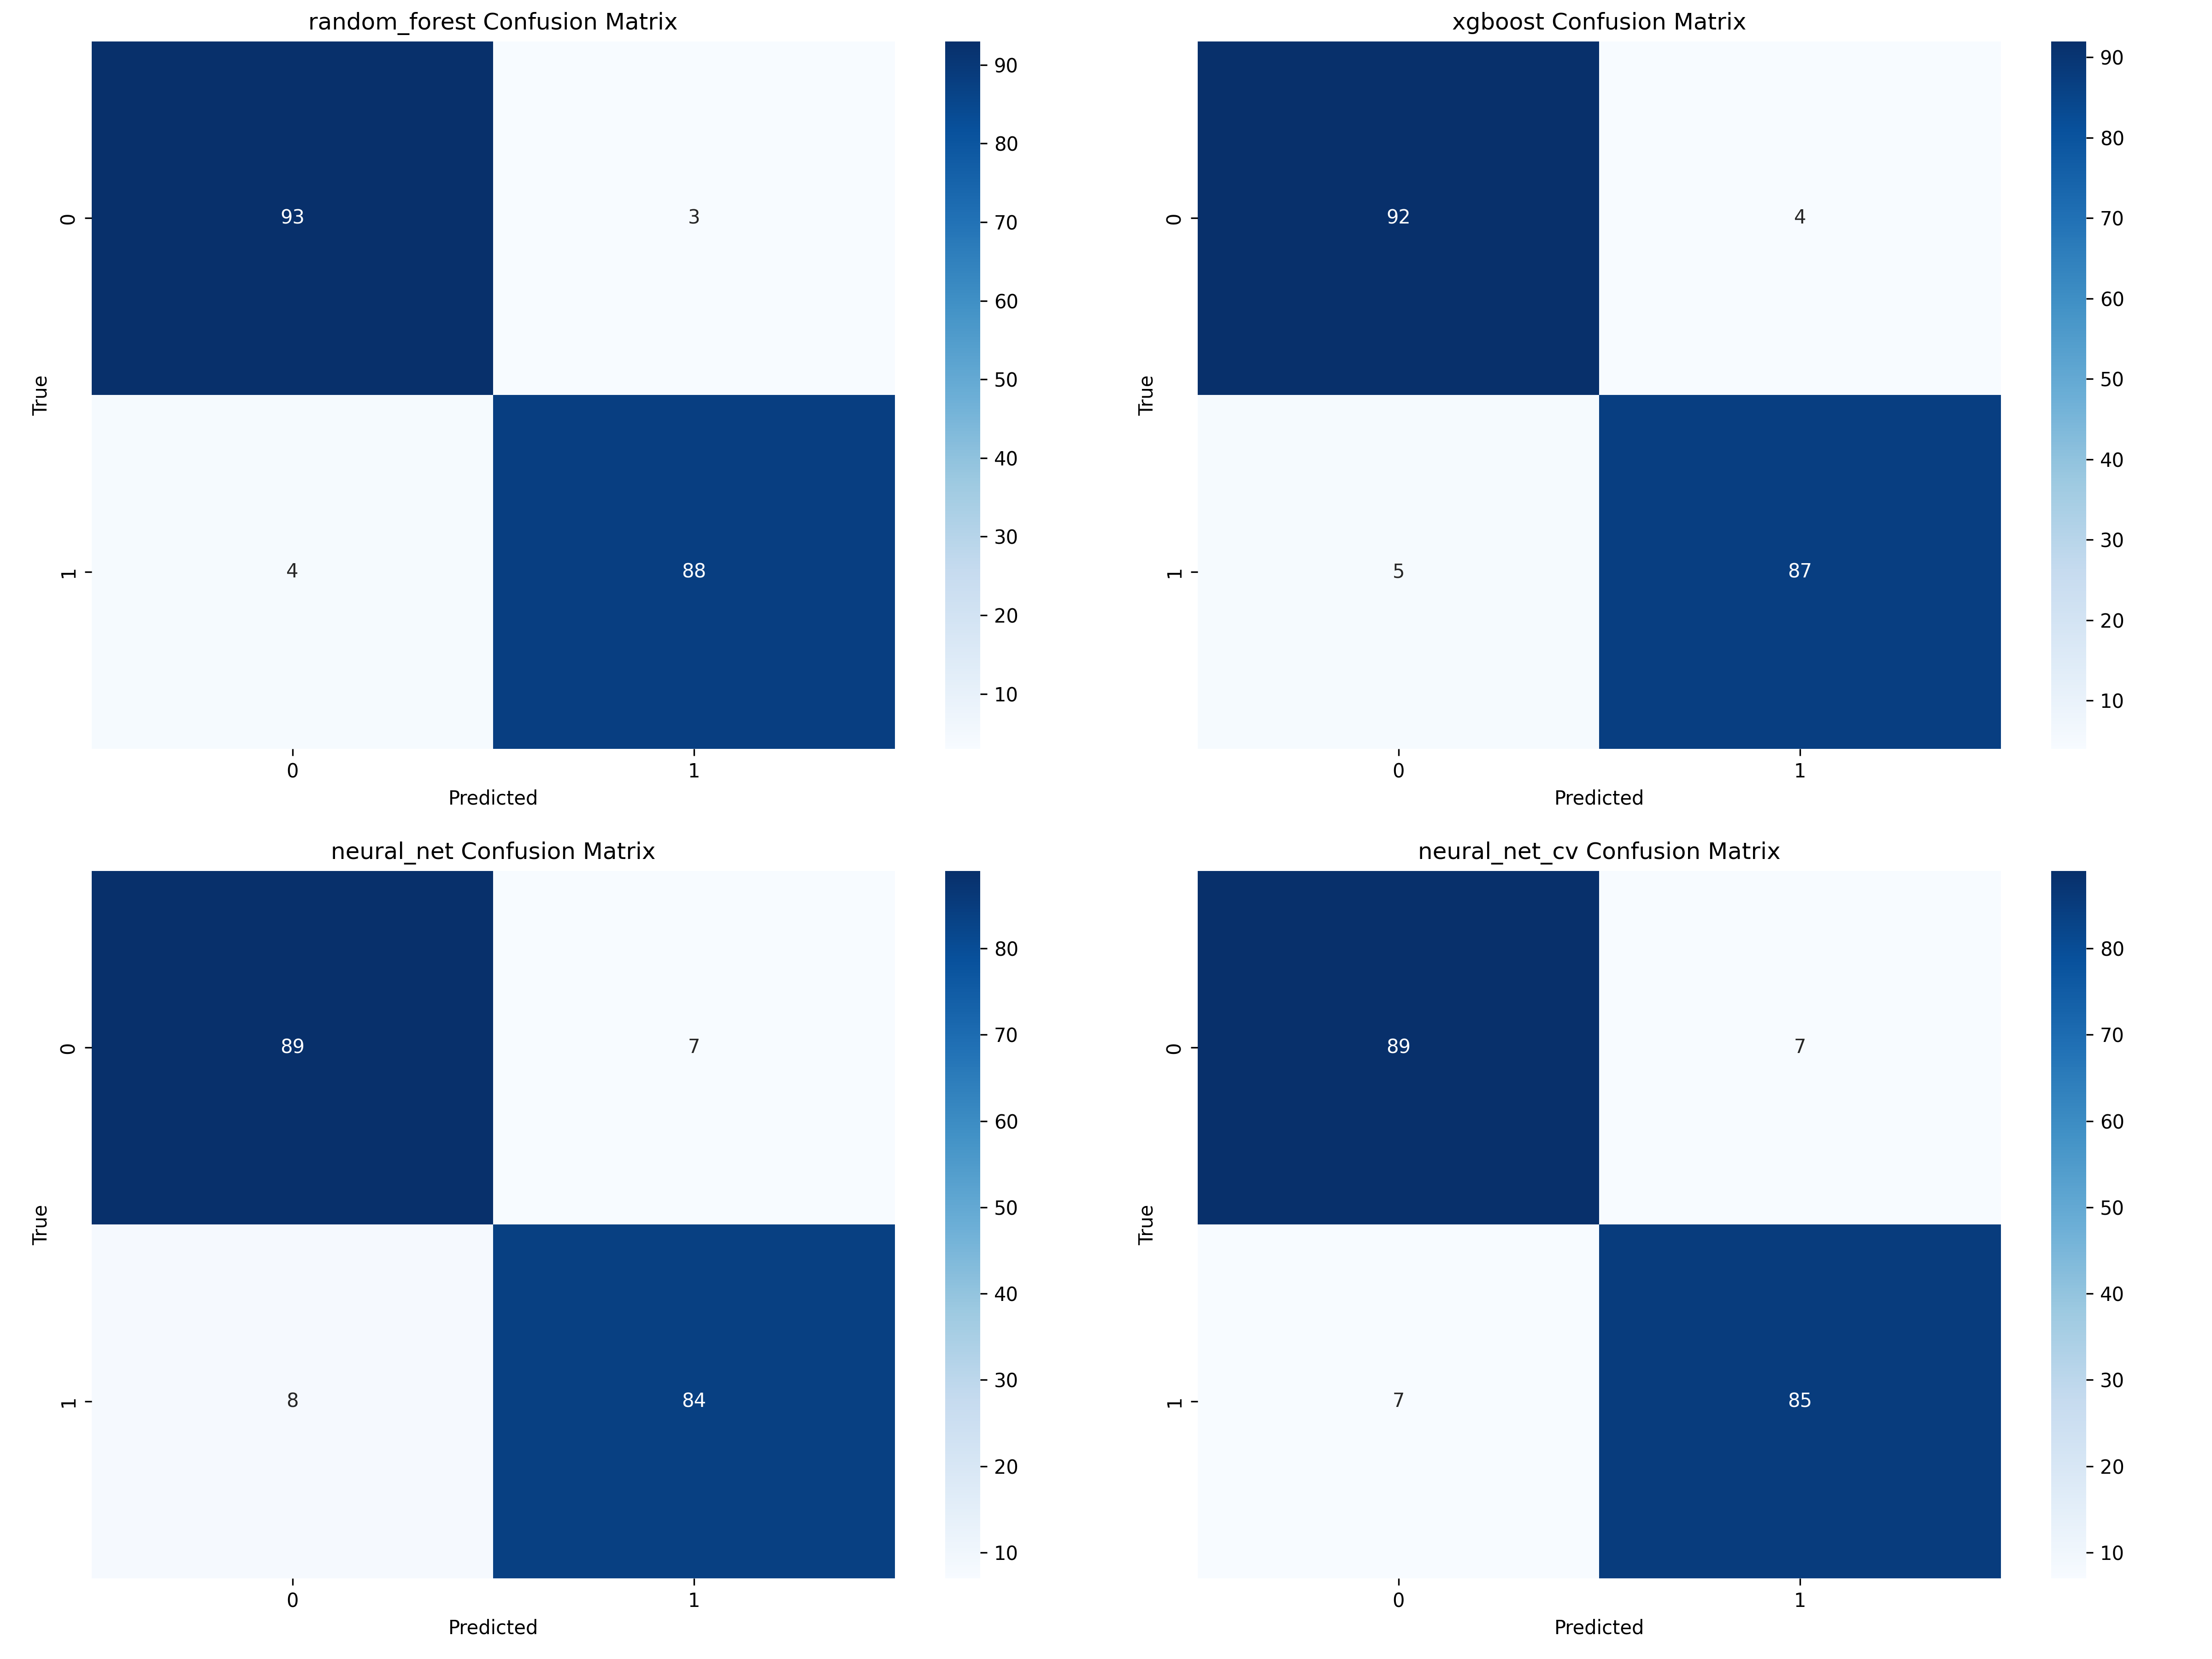
\includegraphics[width=0.8\textwidth]{images/confusion_matrices_comparison.png}
    \caption{مقایسه ماتریس‌های درهم‌ریختگی برای سه مدل پیشنهادی}
\end{figure}

\subsection{منحنی‌های ROC و Precision-Recall}
منحنی‌های ROC و Precision-Recall، ابزارهای مهمی برای ارزیابی جامع عملکرد طبقه‌بندی‌کننده‌ها هستند. در این پژوهش، این منحنی‌ها برای هر سه مدل رسم و مقایسه شده‌اند.

\begin{figure}[h]
    \centering
    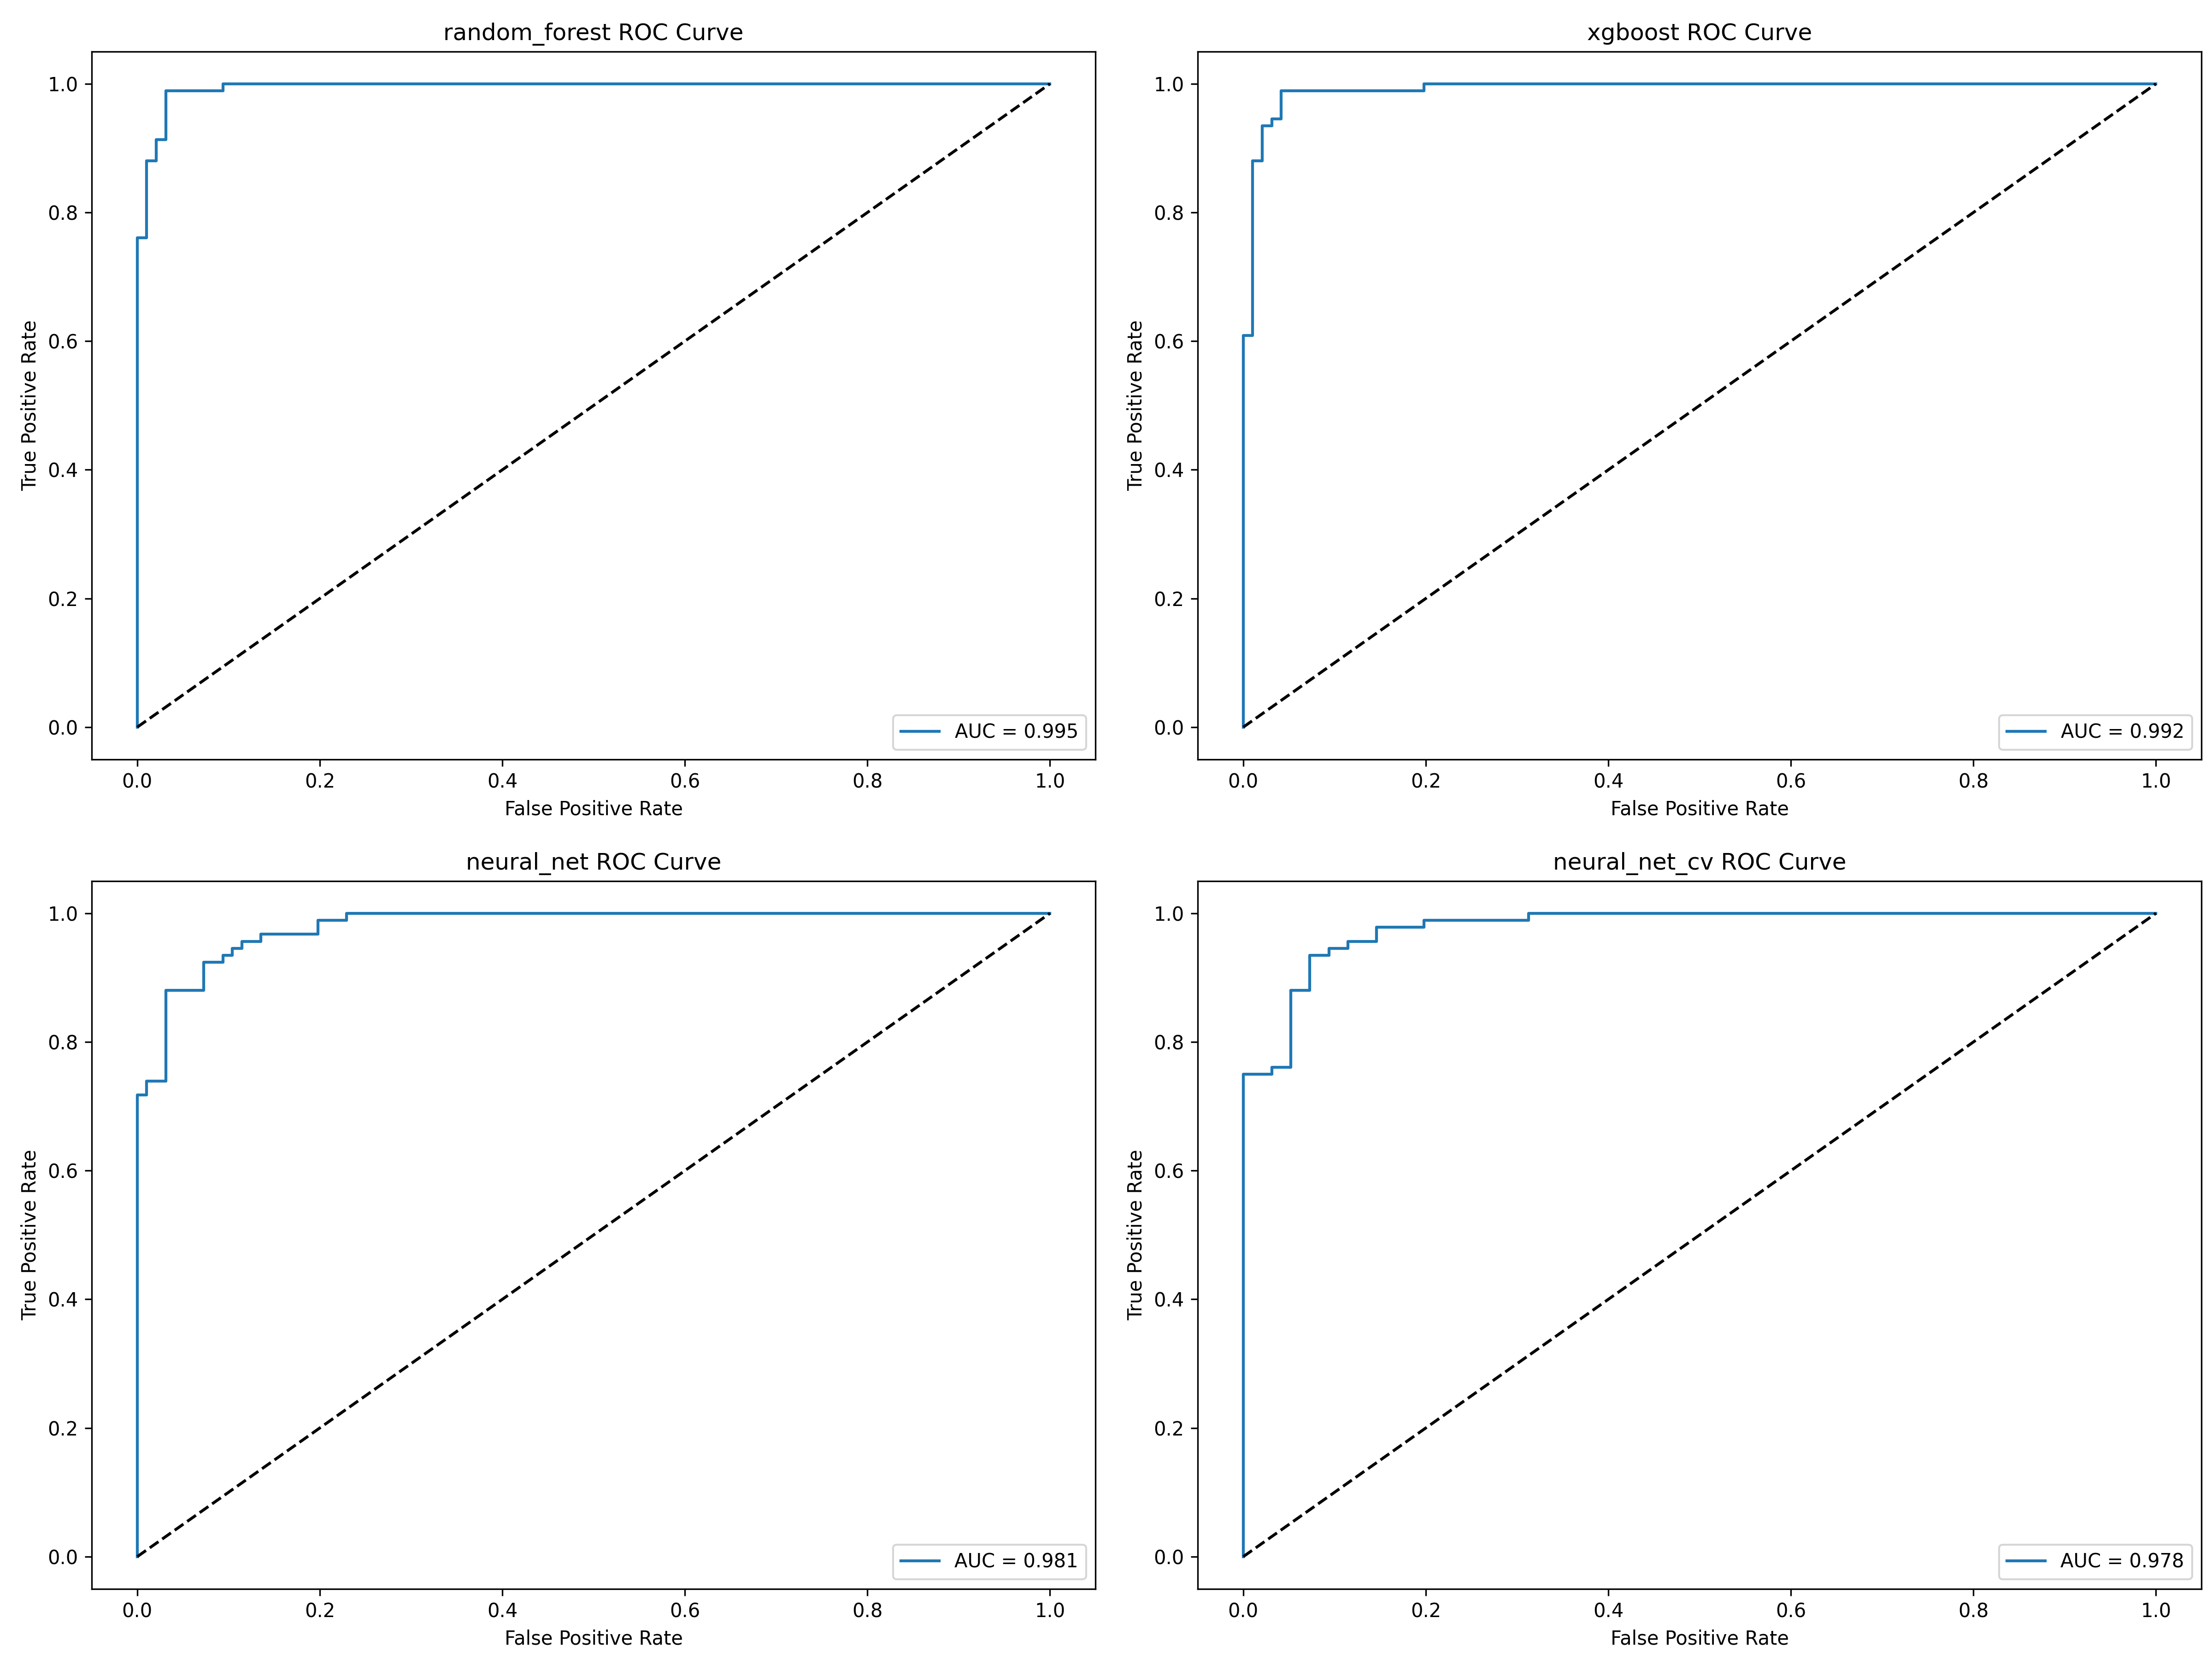
\includegraphics[width=0.48\textwidth]{images/roc_curves.png}
    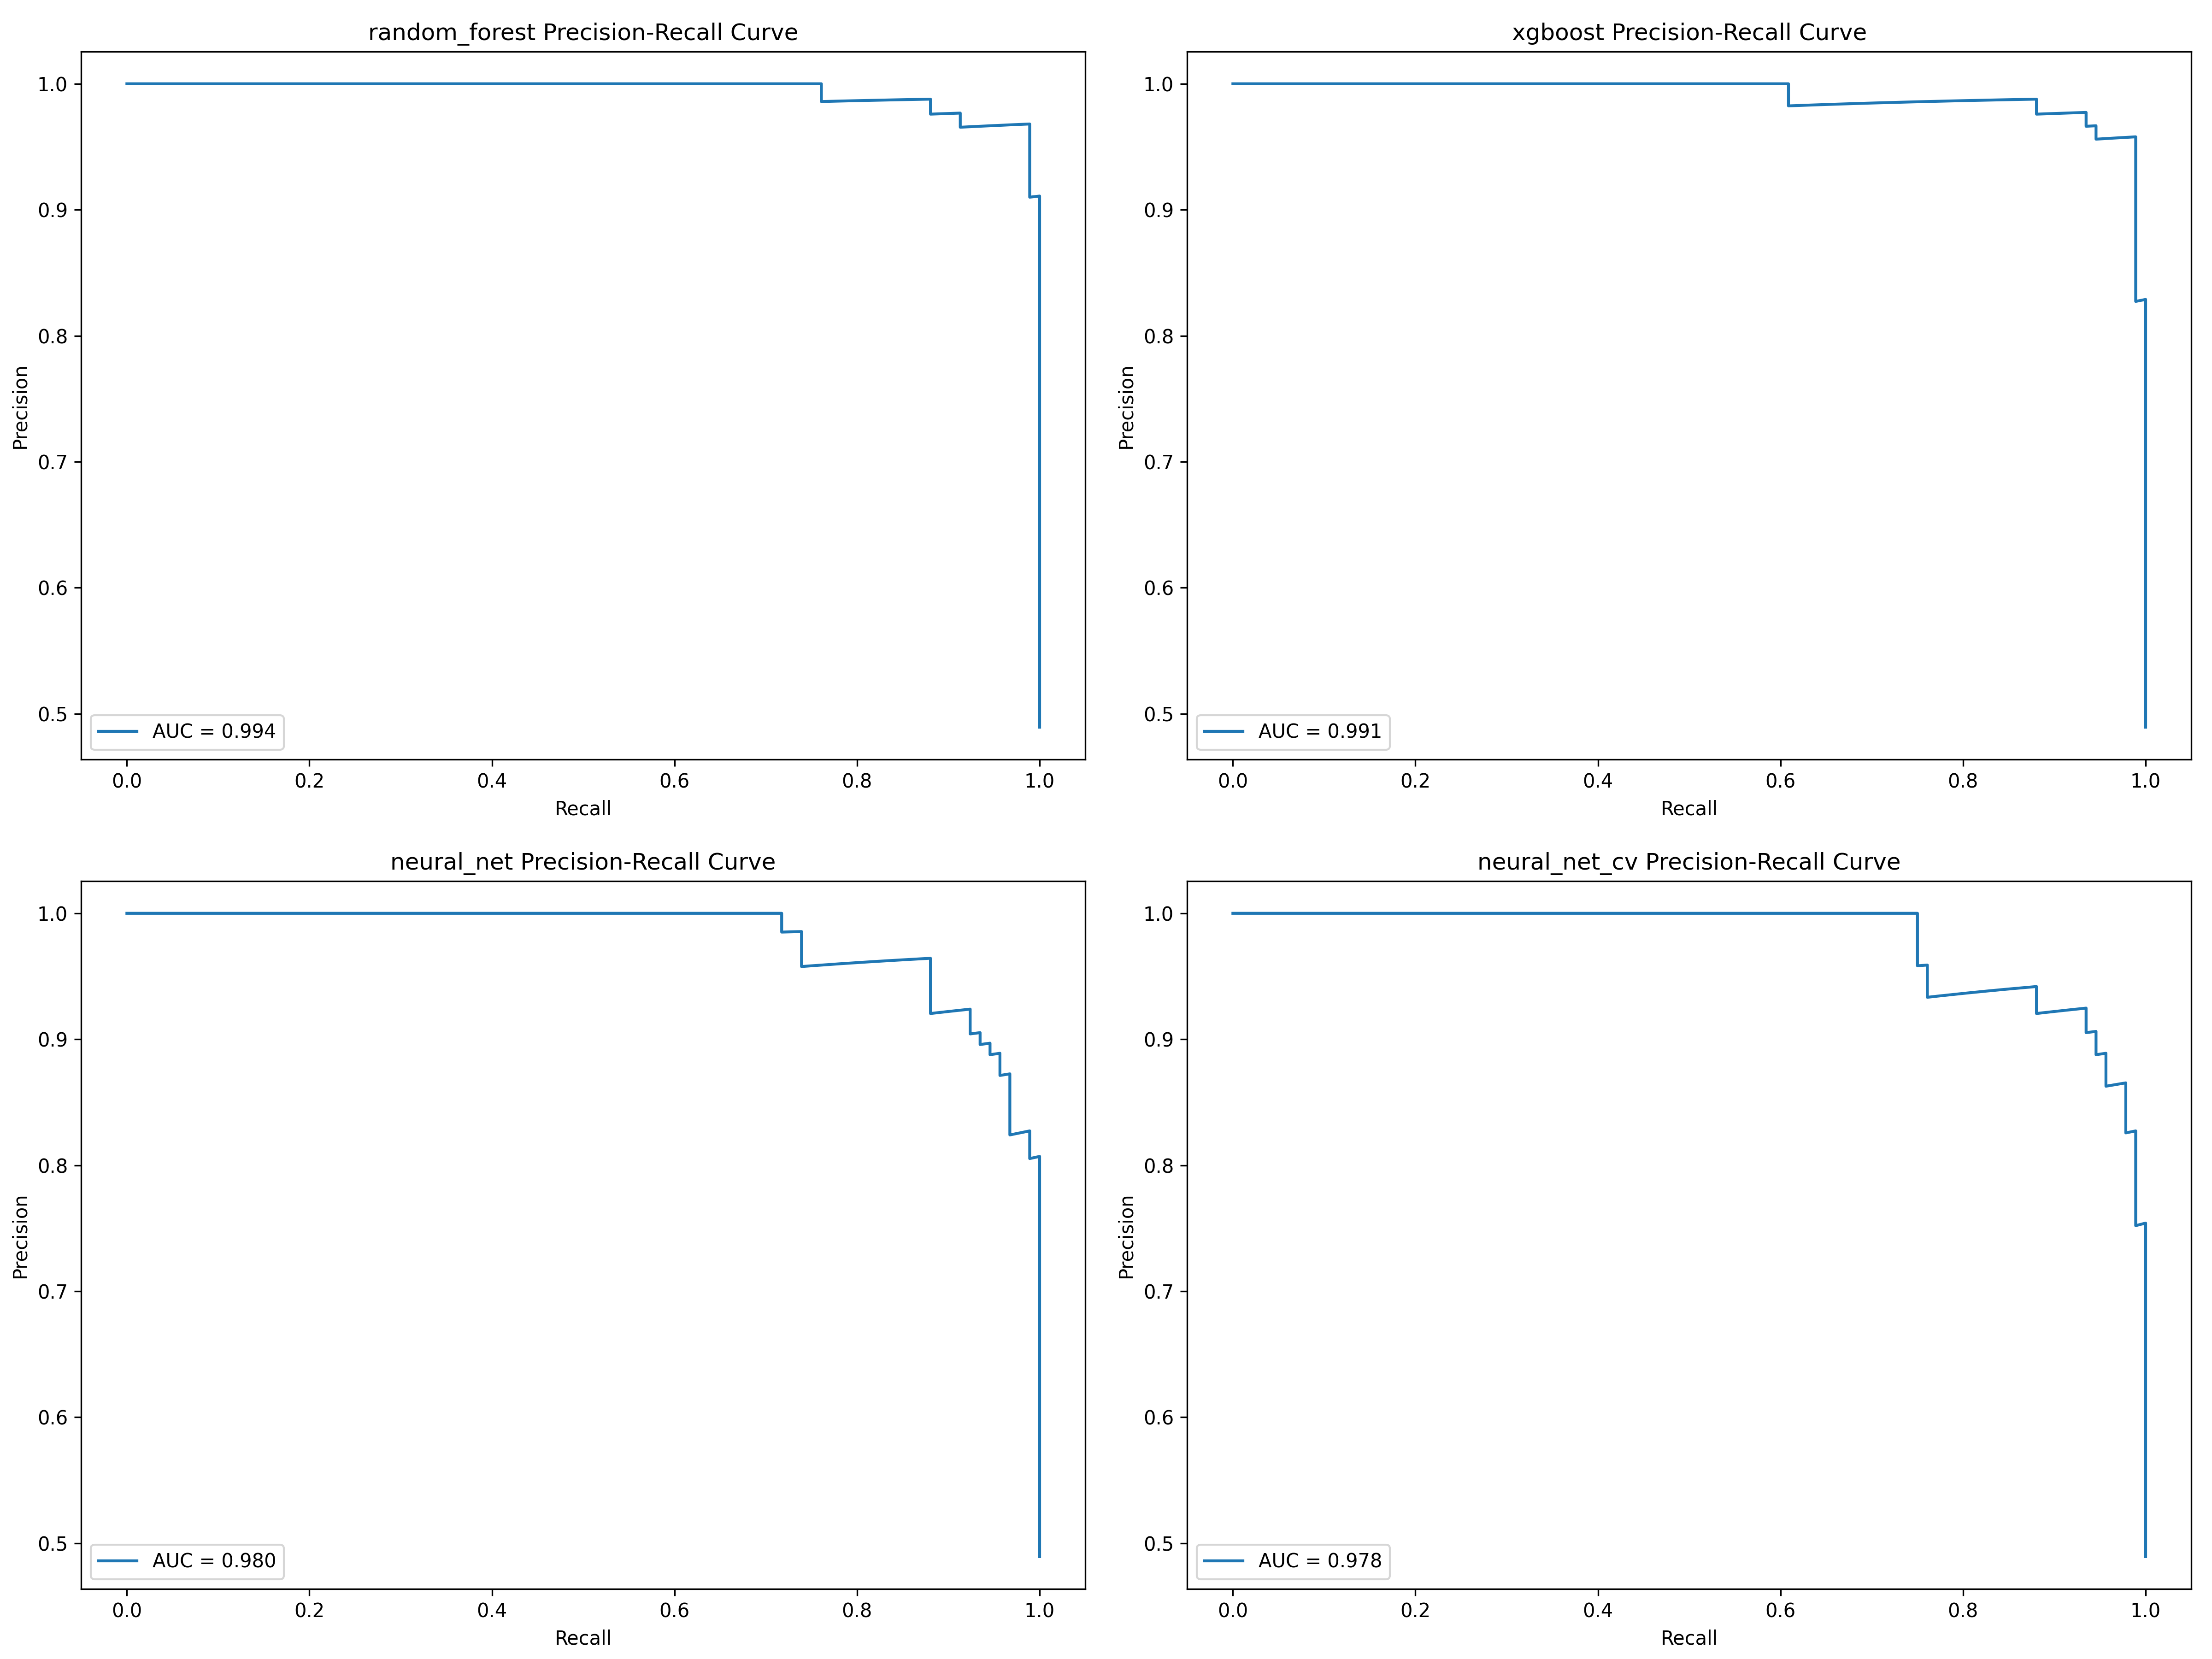
\includegraphics[width=0.48\textwidth]{images/pr_curves.png}
    \caption{منحنی‌های ROC (سمت چپ) و Precision-Recall (سمت راست) برای مدل‌های پیشنهادی}
\end{figure}

\section{تحلیل نتایج و بحث}
یافته‌های اولیه نشان می‌دهد که هر سه مدل عملکرد قابل قبولی در تشخیص باج‌افزارها داشته‌اند، اما تفاوت‌های قابل توجهی در جنبه‌های مختلف عملکرد آن‌ها وجود دارد.

\subsection{مقایسه نقاط قوت و ضعف مدل‌ها}
\begin{itemize}
    \item \textbf{رندوم فارست:} بالاترین دقت کلی را در میان مدل‌ها داشته و از نظر تفسیرپذیری نیز برتری دارد. همچنین عملکرد پایداری در تمام اجراها نشان داده است. با این حال، از نظر حساسیت (Recall) در برخی موارد ضعیف‌تر از XGBoost عمل کرده است.

    \item \textbf{XGBoost:} بهترین عملکرد را از نظر حساسیت داشته و سریع‌ترین زمان استنتاج را نیز به خود اختصاص داده است. این ویژگی، XGBoost را برای کاربردهای بلادرنگ مناسب می‌سازد. چالش اصلی این مدل، تنظیم دقیق پارامترها برای جلوگیری از بیش‌برازش است.

    \item \textbf{شبکه عصبی (MLP):} اگرچه از نظر دقت کلی پایین‌تر از دو مدل دیگر قرار دارد، اما در برخی نمونه‌های پیچیده که الگوهای غیرخطی دارند، عملکرد بهتری نشان داده است. همچنین بالاترین میانگین دقت (Average Precision) را داشته که نشان‌دهنده قابلیت خوب آن در ارائه احتمالات پیش‌بینی معنادار است.
\end{itemize}

\subsection{الگوهای اشتباه مشترک}
تحلیل نمونه‌هایی که توسط هر سه مدل به اشتباه طبقه‌بندی شده‌اند، نشان می‌دهد که برخی الگوهای خاص برای همه مدل‌ها چالش‌برانگیز بوده‌اند:

\begin{itemize}
    \item فایل‌های با رفتار مشابه باج‌افزار اما ماهیت خوش‌خیم (مانند برخی نرم‌افزارهای فشرده‌سازی)
    \item باج‌افزارهای با تکنیک‌های پنهان‌سازی پیشرفته که الگوی دسترسی به فایل آن‌ها شباهت زیادی به نرم‌افزارهای عادی دارد
    \item فایل‌هایی با تعداد بسیار کم عملیات دسترسی که داده‌های کافی برای تحلیل الگو فراهم نمی‌کنند
\end{itemize}

شناسایی این الگوها می‌تواند به طراحی ویژگی‌های جدید و بهبود مدل‌ها در تحقیقات آینده کمک کند.

\section{راهکارهای پیشنهادی و توسعه‌های آتی}
با توجه به نتایج به‌دست آمده و تحلیل نقاط قوت و ضعف مدل‌های مختلف، جهت بهبود عملکرد سیستم تشخیص باج‌افزار پیشنهادات زیر ارائه می‌شود:

\begin{itemize}
    \item \textbf{افزایش حجم و تنوع داده‌ها:} گردآوری داده‌های بیشتر از منابع متنوع می‌تواند به تعمیم‌پذیری بهتر مدل‌ها و کاهش اثر نویز در داده‌های واقعی کمک کند.
    \item \textbf{بهینه‌سازی استخراج ویژگی‌ها:} توسعه و پیاده‌سازی روش‌های پیشرفته‌تر در مهندسی ویژگی‌ها، از جمله استفاده از تکنیک‌های یادگیری عمیق جهت استخراج ویژگی‌های سطح بالاتر، می‌تواند به شناسایی الگوهای پنهان و پیچیده در رفتار باج‌افزارها یاری رساند.
    \item \textbf{استفاده از مدل‌های ترکیبی (Ensemble):} ترکیب مدل‌های مختلف مانند رندوم فارست، XGBoost و شبکه عصبی می‌تواند از نقاط قوت هر یک بهره‌مند شده و عملکرد نهایی را بهبود بخشد.
    \item \textbf{تنظیم دقیق‌تر هایپرپارامترها:} بهره‌گیری از الگوریتم‌های بهینه‌سازی پیشرفته مانند بهینه‌سازی بیزی در تنظیم دقیق پارامترهای مدل‌ها، می‌تواند فضای جستجو را هوشمندانه‌تر کرده و عملکرد نهایی را ارتقا دهد.
    \item \textbf{استفاده از یادگیری انتقالی:} پیاده‌سازی مدل‌های پیش‌آموزش‌دیده در حوزه‌های مرتبط و تطبیق آن‌ها با مسئله تشخیص باج‌افزار می‌تواند به تسریع روند آموزش و بهبود عملکرد در شرایط داده‌های کم کمک کند.
\end{itemize}

\subsection{چالش‌های آتی}
با وجود پیشرفت‌های حاصل در این پژوهش، چالش‌هایی همچنان باقی مانده است که می‌تواند موضوع تحقیقات آینده قرار گیرد:
\begin{itemize}
    \item \textbf{تطبیق با داده‌های دنیای واقعی:} داده‌های واقعی ممکن است شامل نویزهای پیچیده‌تر و تغییرات پویاتر باشند که نیازمند مدل‌هایی با تعمیم‌پذیری بالا هستند.
    \item \textbf{زمان استنتاج در کاربردهای بلادرنگ:} کاهش زمان استنتاج و بهبود سرعت پردازش به ویژه در سیستم‌های بلادرنگ از اهمیت ویژه‌ای برخوردار است.
    \item \textbf{ارتقاء تعمیم‌پذیری مدل‌ها:} ارزیابی و بهبود عملکرد مدل‌های آموزش‌دیده در شرایط خارج از مجموعه داده‌های آموزشی فعلی جهت شناسایی تغییرات در الگوهای حملات یک چالش اساسی است.
\end{itemize}

\subsection{پیشنهادات برای تحقیقات آینده}
به منظور ارتقاء سیستم تشخیص باج‌افزار و رفع چالش‌های موجود، پیشنهاد می‌شود:
\begin{itemize}
    \item بررسی اثر ترکیب مدل‌های مختلف (ensembling) بر عملکرد کلی سیستم و کاهش نقاط ضعف هر مدل به‌صورت مجزا
    \item توسعه الگوریتم‌های یادگیری عمیق با معماری‌های پیشرفته‌تر و بهره‌گیری از تکنیک‌های یادگیری انتقالی برای استخراج ویژگی‌های پیچیده
    \item تحلیل عمیق‌تر داده‌های رفتاری با استفاده از روش‌های تحلیل سری زمانی و مدل‌های گرافی به منظور استخراج الگوهای پنهان در فعالیت‌های فایل‌ها
    \item ارزیابی سیستم در محیط‌های عملی و واقعی جهت سنجش عملکرد در شرایط غیر ایده‌آل و ارائه راهکارهای بهبود سازگار با تغییرات محیطی
\end{itemize}

این راهکارها و پیشنهادات می‌تواند به عنوان مبنایی برای تحقیقات آتی در حوزه تشخیص باج‌افزار مورد استفاده قرار گیرد و زمینه ارتقاء دقت و کارایی سیستم‌های امنیتی در مواجهه با تهدیدهای نوین را فراهم آورد.
